% ----------------------------------------------------------------
% achemso --- Support for submissions to American Chemical
%  Society journals
% Maintained by Joseph Wright
% E-mail: joseph.wright@morningstar2.co.uk
% Originally developed by Mats Dahlgren
%  (c) 1996-98 by Mats Dahlgren
%  (c) 2007-2008 Joseph Wright
% Released under the LaTeX Project Public license v1.3c or later
% See http://www.latex-project.org/lppl.txt
% 
% Part of this bundle is derived from cite.sty, to which the
% following license applies:
%   Copyright (C) 1989-2003 by Donald Arseneau
%   These macros may be freely transmitted, reproduced, or
%   modified provided that this notice is left intact.
% ----------------------------------------------------------------
% 
% The achemso bundle provides a LaTeX class file and BibTeX style
% file in accordance with the requirements of the American
% Chemical Society.  The files can be used for any documents, but
% have been carefully designed and tested to be suitable for
% submission to ACS journals.
% 
% The bundle also includes the natmove package.  This package is
% loaded by achemso, and provides automatic moving of superscript
% citations after punctuation.




\documentclass[
%journal=ancac3, % for ACS Nano
%journal=acbcct, % for ACS Chem. Biol.
journal=jacsat, % for undefined journal
manuscript=article]{achemso}



\usepackage[utf8]{inputenc}
%\usepackage{lmodern}

%\renewcommand*\familydefault{\sfdefault} 


% https://tex.stackexchange.com/questions/121061/working-with-arial-or-helvetica-fonts#121063
%\usepackage[scaled]{helvet}
%\renewcommand\familydefault{\sfdefault} 
%\usepackage[T1]{fontenc}


\renewcommand{\familydefault}{\sfdefault}
\usepackage[scaled=1]{tgheros}
\usepackage[helvet]{sfmath}
\everymath={\sf}
\usepackage[T1]{fontenc}



%\usepackage[T1]{fontenc}
%\usepackage{lmodern}
%\usepackage[version=3]{mhchem} % Formula subscripts using \ce{}

%\newcommand*{\mycommand}[1]{\texttt{\emph{#1}}}


\author{Carl Mathias Kobel}

\affiliation[Unknown University]
{BiRC, AU}

\email{kobel@pm.me}

\title[\texttt{achemso} demonstration]
{Bachelor Project: Copy Number Variation of Ampliconic Regions on Hominid X and Y chromosomes}

\begin{document}

\begin{abstract}
By mapping the genomes of a few Chimpanzee and Gorilla individuals, we measured the copy number variation of a few genes that were assumed to be ampliconic based on human trials.
\end{abstract}

\clearpage
%%%%%%%%%%%%%%%%%%%%%%%%%%%%%%%%%%%%%%%%%%%%%%%%%%%%% Introduction
\section{Introduction}
No idea how they evolved > how they diverged between human, chimp and gorilla
Were they ampliconic 
Did the ampliconic genes become amplified in the human lineage or in the great apes?
What drives ampliconic gene evolution


\subsection{Outline}



%Citation of Einstein paper~\cite{doi:10.1093/molbev/msi198}.

\clearpage
%%%%%%%%%%%%%%%%%%%%%%%%%%%%%%%%%%%%%%%%%%%%%%%%%%%%% Method
\section{Method}

\subsection{Overview}
The pipeline (Figure \ref{fig:pipeline}) of this project consists of several parts, all originating from \textit{Lucotte et al.\cite{LucotteDyn}}. Firstly, an artificial chromosome with ampliconic candidates was assembled for each species, for each of their sex chromosomes. Later, reads of the genomes were mapped upon the artificial chromosome, and the copy number was estimated with a non-ampliconic control.
%\def\code#1{\texttt{#1}}


\begin{figure}
  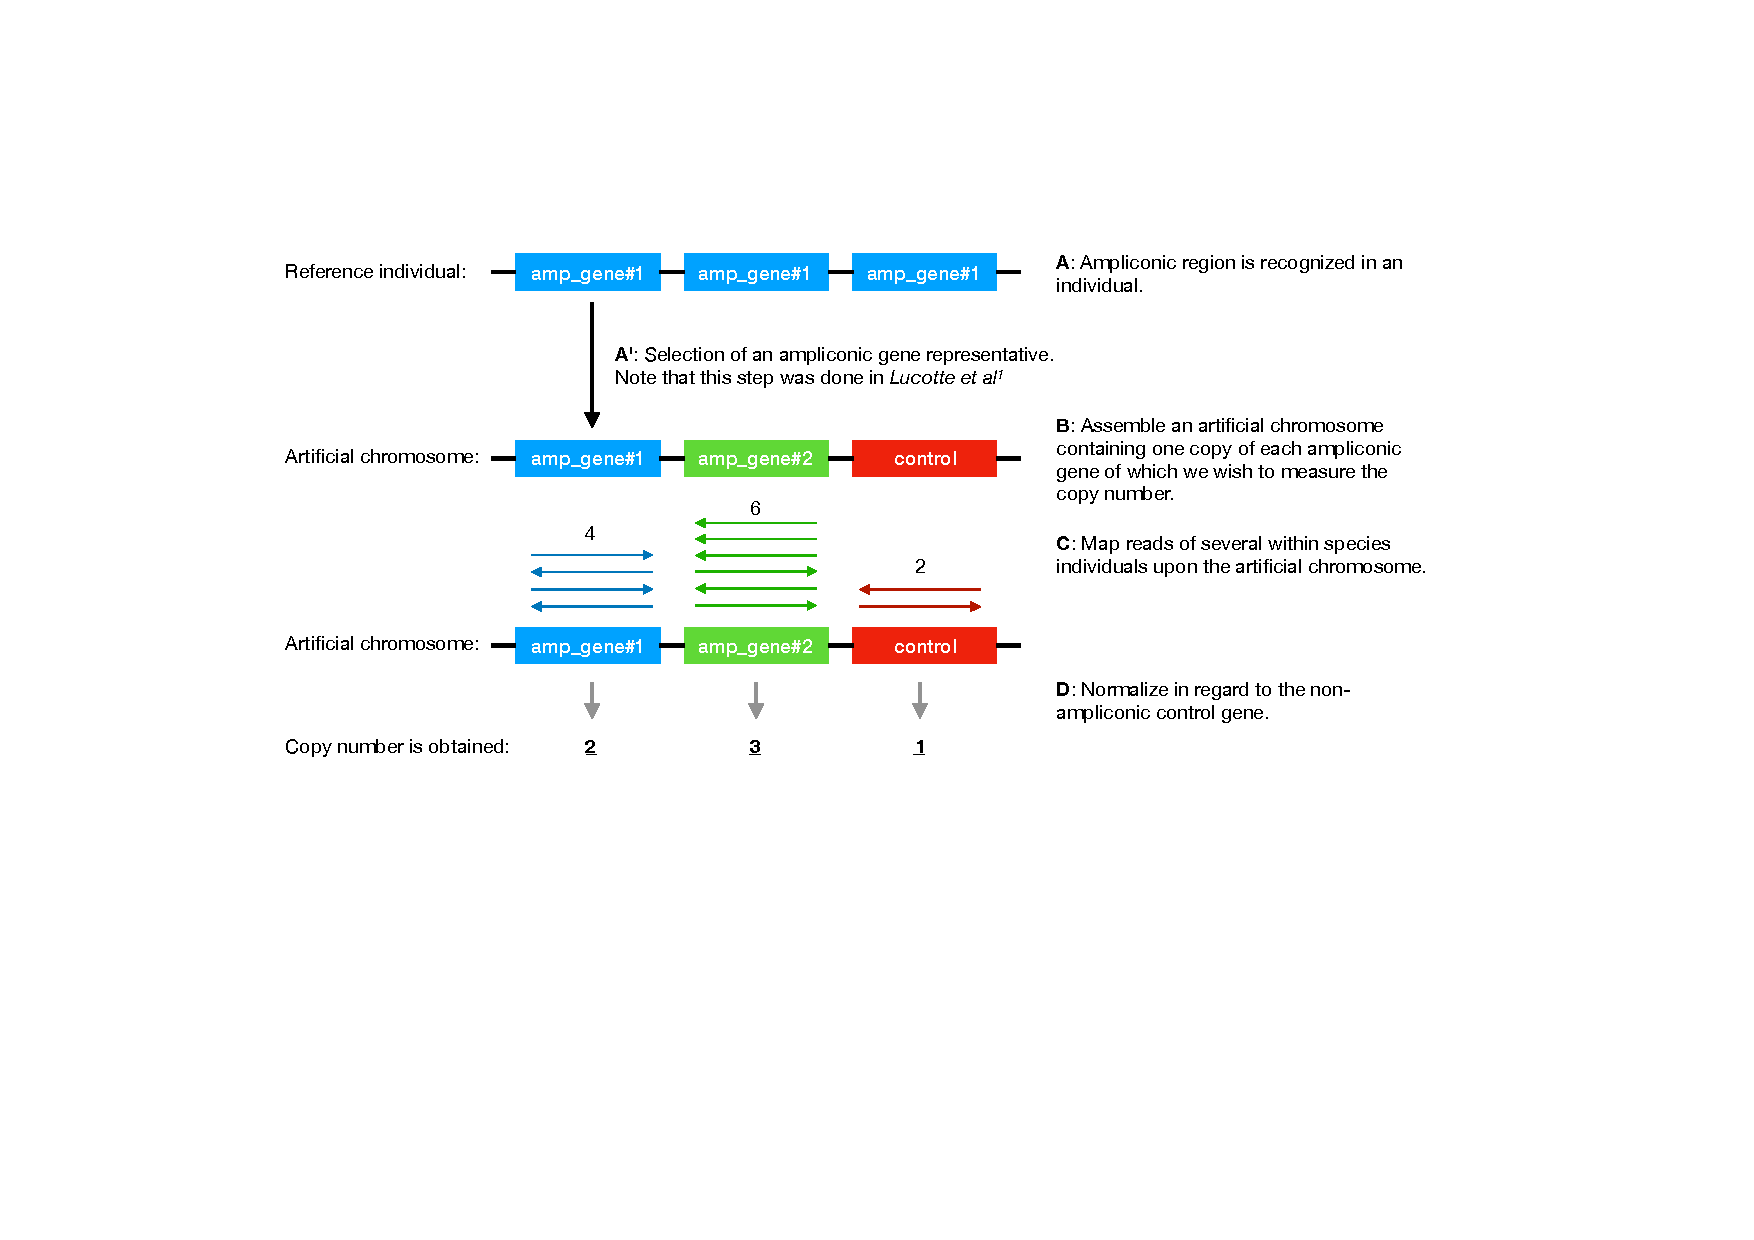
\includegraphics[width=\linewidth]{illustrations/figure_pipeline.pdf}
  \caption{A complete overview of the pipeline.}
  \label{fig:pipeline}
\end{figure}



\subsection{Assembly of artificial chromosome}
For assembly of the artificial chromosomes (artificial chromosomes) we selected the human genes showing ampliconic behaviour from \textit{Lucotte et al.\cite{LucotteDyn}}. These genes are selected visually from dotplots. We searched for orthologs in chimpanzee (reference: Pan\_tro\_3.0) and gorilla (reference: gorGor4) for the associated human genes in the Ensembl genome browser. Only orthologs with a subject/query identical factor of more than 0.5 were included (see Table \ref{tab:orthologs}). When orthologs were not found in Ensembl, we blasted the human genes against the chimpanzee and gorilla references \texttt{blastn -subject <reference>.fa -query <human\_gene>.fa -out output.txt} and again only selected regions with a subject/query identical factor of more than 0.5. The orthologs found on ensembl were downloaded directly as fasta files. The orthologs found with blast were cut out of the reference with \texttt{samtools faidx <reference>.fa <chromosome>:<start>-<end>}. The files were later merged into complete artificial chromosomes with \texttt{cat *.fa > <artificial\_ chromosome>.fa}. These artificial chromosomes (chimpanzee X, chimpanzee Y and gorilla X) were then put into the read-mapping pipeline presented in the next part. Several problems occured in the assembly of the artificial chromosomes. We checked coherence between Ensembl and BLAST results with GAGE4 in gorilla. The Query \%id and BLAST Identities are on par, but the length fraction is far off. This may be due to the way the human ampliconic regions were chosen. The human ampliconic regions from \textit{Lucotte et al.\cite{LucotteDyn}} has a length of 7330bp whereas the corresponding gene on Ensembl has a length of 15285bp. The remedy could be to blast the human genes from Ensembl against the chimpanzee and gorilla references.



\begin{table}
\footnotesize
    \begin{center}
        \begin{tabular}{  l | c | l | p{1.8cm} | p{1.8cm} | p{1.8cm} | p{1.8cm} }
                \textbf{Species} & \textbf{Chr.} & \textbf{Gene} & \textbf{Ensemble Query id\%} & \textbf{Ensembl length fraction} & \textbf{BLAST Identities} & \textbf{BLAST length fraction} \\ 
                \hline
                    Chimpanzee & X & CT45A5 & 0.96 & 1.81 & - & - \\ 
                    Chimpanzee & X & CT47A4 & 0.92 & 1.15 & - & - \\ 
                    Chimpanzee & X & GAGE4 & 0.82 & 2.27 & - & - \\ 
                    Chimpanzee & X & OPN1LW & - & - & 0.98 & 0.95 \\ 
                    Chimpanzee & X & SPANXB1 & 0.68 & 0.85 & - & - \\ 
                    Chimpanzee & X & DMD (control) & 0.99 & 1.00 & - & - \\ 
                    \hline
                    Gorilla & X & CT45A5 & 0.78 & 0.76 & - & - \\ 
                    Gorilla & X & CT47A4 & 0.80 & 0.31 & - & - \\ 
                    Gorilla & X & GAGE4 & 0.89 & 2.09 & 0.90 & 0.51 \\ 
                    Gorilla & X & SPANXB1 & 0.67 & 1.75 & - & - \\ 
                    Gorilla & X & DMD (control) & 0.99 & 1.00 & - & - \\ 
                    \hline
                    Chimpanzee & Y & BPY2 & 0.98 & 0.19 & - & - \\ 
                    Chimpanzee & Y & CDY & 0.97 & 0.77 & - & - \\ 
                    Chimpanzee & Y & PRY & 0.97 & 0.52 & - & - \\ 
                    Chimpanzee & Y & RBMY1A1 & 0.91 & 0.32 & - & - \\ 
                    Chimpanzee & Y & TSPY & 0.90 & 1.43 & - & - \\ 
                    Chimpanzee & Y & XKRY & - & - & 0.98 & 1.00 \\ 
                    Chimpanzee & Y & AMELY (control) & 0.98 & 1.00 & - & - \\ 
        \end{tabular}
        \caption{Table of orthologs chosen for assembly of the artificial chromosomes for the respective species. Query id\% is the percentage of the human sequence matching the sequence of the orthologue. Length fraction denotes the length of the orthologue relative to the original (human) sequence. Identities denotes the fraction of similar nucleotides in the pairwise alignment. Orthologue candidate genes with a Query id\% < 0.5 or length fraction < 0.5 were discarded. See the full table including discarded samples at google drive\cite{gdriveorthoac}}
        \label{tab:orthologs}
    \end{center}
\end{table}

\normalsize


\subsection{Mapping of artificial chromosomes upon genomes}


The following part of the pipeline was written into a workflow with gwf-org\cite{gwforg} in order to support parametric inputs, easing reproducibility. The original code from \textit{Lucotte et al.\cite{LucotteDyn}} was rewritten from gwf v0.7 to v1.2.1 and python v2.7 to 3.6 in order to use newer functionality in the packages. In this process, much of the code was also reorganized in such a way that all input parameters were concentrated in one spot, such that the pipeline can easily be used for different batches of individuals, which may be needed in order to produce results with a higher statistical power. The takes in a number of individuals (grouped in species) and their genomes, and an artificial chromosome as reference. This is done by passing a dictionary with various elements to the workflow. When all the input parameters are parsed from various text files (??explain), it indexes the genomes and starts mapping each phase of the genome upon the artificial chromosome. Since the individuals might have been sequenced several times independently (??maybe from various tissues - who knows??), and these sequences are all included, we merge the sequence alignments (BAM-files) into one per individual. For quality control, we filter with Sambamba\cite{doi:10.1093/bioinformatics/btv098}: \texttt{(mapping\_quality >= 50) and (cigar =~ /100M/) and ([NM] < 3)}. We then calculate the read depth with SAMtools\cite{Li:2009:SAF:1613280.1613286}. Because the distribution is not necessarily symmetric, we take the median of the read depth across all positions in the gene. This median number is what we subsequently regard as the copy number. In order to normalize the copy number of each gene, we divide by the copy number of the controls. In case of the X chromosome, we selected DMD as a control gene, since it is known to be non-ampliconic (in humans). For the Y chromosome AMELY is selected for the same reason. Surely, it would have made a lot of sense to include many more control genes, as there is no reason to believe that DMD and AMELY might not be non-ampliconic, other than the fact that their distributions look very limited (See the discussion section??).

\subsection{Visualization}


\clearpage
%%%%%%%%%%%%%%%%%%%%%%%%%%%%%%%%%%%%%%%%%%%%%%%%%%%%% Results
\section{Results}

\subsection{Visual overview}

New float types are automatically set up by the class file. The
means graphics are included as follows (scheme \ref{sch:example}).  As
illustrated, the float is ``here'' if possible.
\begin{scheme}
  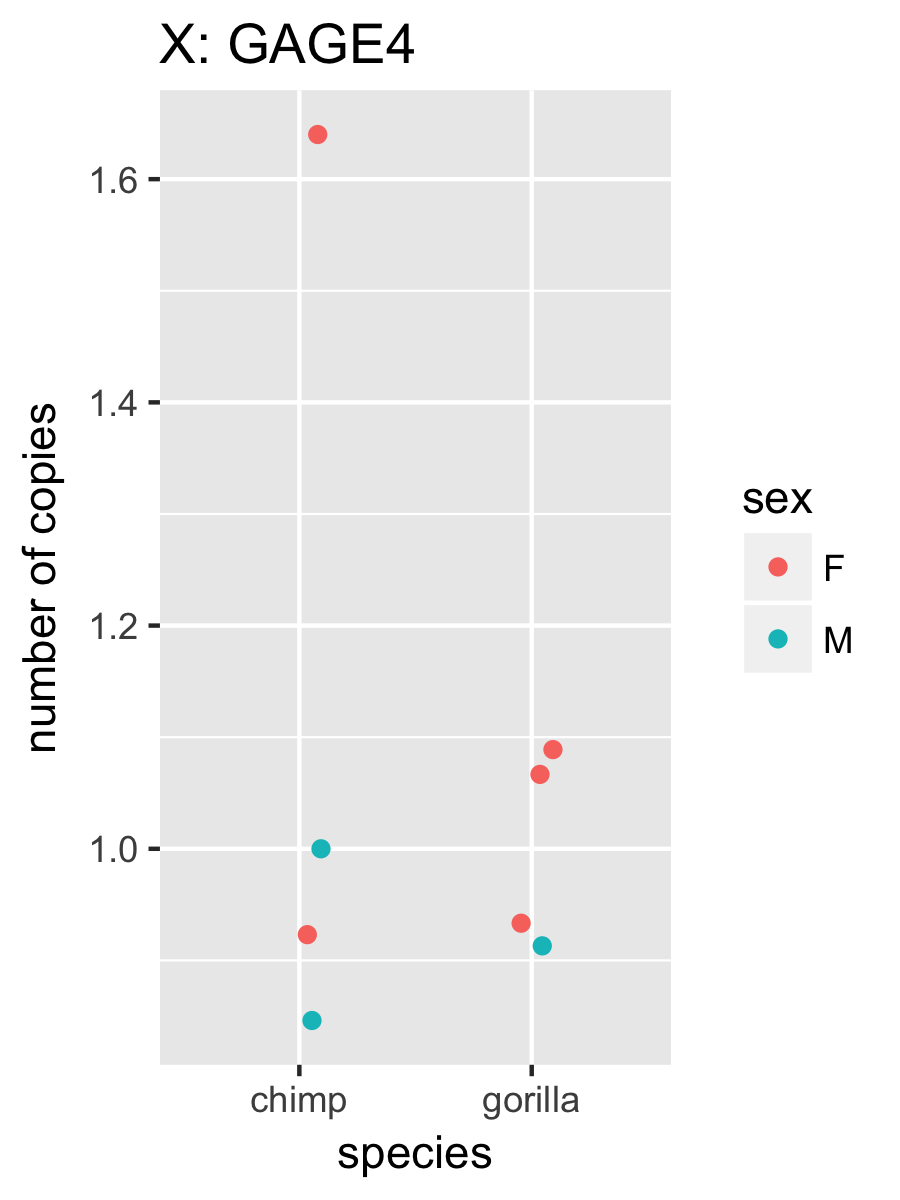
\includegraphics[height=10cm]{figure_X_gene_GAGE4.png}
  \caption{An example graphics}
  \label{sch:example}
\end{scheme}


\clearpage
%%%%%%%%%%%%%%%%%%%%%%%%%%%%%%%%%%%%%%%%%%%%%%%%%%%%% Discussion
\section{Discussion}

What can we really conclude?
Take basis in examples from the results.
Try and make it sound like there is 



% references
\bibliography{sample}

\end{document}
